\documentclass[12pt]{article}
% ====== Page Layout and Basic Formatting ======
\usepackage[left=1.0in,right=1.0in,top=1.0in,bottom=1.0in]{geometry}
\usepackage{setspace}
\doublespacing
\usepackage{fancyhdr}
\pagestyle{fancy}
\fancyhf{}
\fancyfoot[C]{\thepage}
\renewcommand{\headrulewidth}{0pt}

% ====== Typography and Fonts ======
\usepackage{lmodern}
\usepackage{microtype}
\usepackage[normalem]{ulem}
\usepackage[T1]{fontenc}

% ====== Section Styling ======
\usepackage{titlesec}
\usepackage[title]{appendix}
\usepackage{titling}
\pretitle{\begin{center}\large\bfseries}
\posttitle{\end{center}}
\preauthor{\begin{center}\normalsize}
\postauthor{\end{center}}
\predate{\begin{center}\normalsize}
\postdate{\end{center}}

% ====== Math Packages ======
\usepackage{amssymb, amsmath, amsfonts, mathtools}
\usepackage{dsfont}
\usepackage{amsthm}
\newtheorem{theorem}{Theorem}
\newtheorem{proposition}{Proposition}
\newtheorem{corollary}{Corollary}
\newtheorem{lemma}{Lemma}
\newtheorem{definition}{Definition}
\newtheorem{hyp}{Hypothesis}
\DeclareMathOperator*{\argmax}{arg\,max}
\DeclareMathOperator*{\argmin}{arg\,min}
\newcommand{\norm}[1]{\left\lVert #1 \right\rVert}
\newcommand{\1}[1]{\mathds{1}\left[#1\right]}

% ====== Table Packages ======
\usepackage{array, booktabs, makecell, cellspace}
\usepackage{siunitx}
\usepackage[flushleft]{threeparttable}
\usepackage{rotating, tabularx}
\usepackage{tabularray}
\UseTblrLibrary{booktabs, siunitx}

% ====== Figure and Caption Packages ======
\usepackage{graphicx, subcaption}
\usepackage{pdflscape, tikz}
\usepackage{caption}
\captionsetup{font=small, labelfont=bf, justification=justified}
\captionsetup[figure]{labelfont=bf}
\usepackage{float}

% ====== List Formatting ======
\usepackage{enumitem}

% ====== Bibliography and Citation (biblatex + biber) ======
\usepackage{xurl}
\usepackage{xcolor}
\definecolor{citationcolor}{RGB}{0, 127, 255}

\usepackage[backend=biber,
            style=authoryear,
            maxcitenames=3,
            mincitenames=1,
            maxbibnames=99,
            giveninits=true,
            uniquename=false,
            uniquelist=true,
            dashed=false,
            urldate=long,
            url=true,
            natbib=true]{biblatex}
\addbibresource{references.bib}

% Citation color settings
\renewcommand*{\nameyeardelim}{\addcomma\space}
\DeclareCiteCommand{\cite}
  {\usebibmacro{prenote}}
  {\usebibmacro{citeindex}%
   \printtext[bibhyperref]{\color{citationcolor}\usebibmacro{cite}}}
  {\multicitedelim}
  {\usebibmacro{postnote}}
\DeclareCiteCommand{\parencite}[\mkbibparens]
  {\usebibmacro{prenote}}
  {\usebibmacro{citeindex}%
   \printtext[bibhyperref]{\color{citationcolor}\usebibmacro{cite}}}
  {\multicitedelim}
  {\usebibmacro{postnote}}

% ====== Custom Column Types ======
\newcolumntype{L}[1]{>{\raggedright\let\newline\\\arraybackslash\hspace{0pt}}m{#1}}
\newcolumntype{C}[1]{>{\centering\let\newline\\\arraybackslash\hspace{0pt}}m{#1}}
\newcolumntype{R}[1]{>{\raggedleft\let\newline\\\arraybackslash\hspace{0pt}}m{#1}}

% ====== Footnote Settings ======
\interfootnotelinepenalty=10000
\setlength{\footnotesep}{0.5cm}

% ====== URL Bleeding Fixes ======
\setcounter{biburllcpenalty}{7000}
\setcounter{biburlucpenalty}{8000}
\setcounter{biburlnumpenalty}{9000}

% ====== Hyperref (loaded second-to-last) ======
\usepackage[hidelinks, breaklinks, colorlinks=true,
            linkcolor=citationcolor, citecolor=citationcolor,
            urlcolor=citationcolor]{hyperref}

% ====== Cleveref (loaded after hyperref) ======
\usepackage[nameinlink]{cleveref}
\crefname{hyp}{Hypothesis}{Hypotheses}
\Crefname{hyp}{Hypothesis}{Hypotheses}

% =============================================================================
\title{Idiosyncratic Volatility and the Cross-Section of Stock Returns:\\
An Update for 1990--2024\thanks{\textbf{Demonstration only --- not for circulation.}
The full code base, data pipeline, and reviewer reports are 
available at \url{https://github.com/mgao6767/mingze-gao/tree/master/teaching/talks/writing-a-paper-in-15min}.}}

\author{Adrian Gao\thanks{Department of Applied Finance, Macquarie Business School,
Macquarie University, NSW 2109, Australia. Email: \href{mailto:mingze.gao@mq.edu.au}{mingze.gao@mq.edu.au}.}}

\date{May 19, 2026}

\begin{document}
\maketitle
\thispagestyle{empty}

% =============================================================================
% DEMONSTRATION BANNER --- not for circulation
% =============================================================================
\begin{center}
\framebox[0.92\textwidth]{%
  \begin{minipage}{0.86\textwidth}\centering
    \textbf{\large Demonstration paper --- not for circulation.}\\[2pt]
    \small This manuscript was produced by Claude Code as a live demonstration
    of AI-assisted empirical research workflows. It is not a finished research
    output. Please do not cite, distribute, or treat as a working paper.
  \end{minipage}%
}
\end{center}
\vspace{0.5em}

% =============================================================================
% ABSTRACT
% =============================================================================
\begin{abstract}
\noindent \singlespacing
\citet{ang2006cross} document that high-idiosyncratic-volatility stocks earn lower
average returns than low-idiosyncratic-volatility stocks --- a puzzle that has
generated two decades of competing explanations. I revisit the puzzle on 1990--2024
US common stocks (1.6 million stock-months, 15{,}030 firms). The unconditional
quintile spread is small and statistically indistinguishable from zero:
$+0.16\%$ per month value-weighted ($t=0.41$). After risk adjustment, however,
the spread reappears: the value-weighted CAPM alpha is $+0.90\%$ per month
($t=2.86$) and the FF3 alpha is $+0.76\%$ ($t=2.96$). The result survives
excluding January, excluding the 2008--09 crisis, and reconstructing
idiosyncratic volatility from FF3 residuals. Adding the Carhart momentum factor
collapses the alpha to $+0.12\%$ ($t=0.61$). In the modern sample, the puzzle
is largely a momentum-related phenomenon.
\end{abstract}

\vspace{1em}
\noindent \textbf{JEL Codes:} G12, G14

\noindent \textbf{Keywords:} idiosyncratic volatility, cross-sectional returns,
asset pricing anomalies, portfolio sorts, Fama-MacBeth

\newpage
\setcounter{page}{1}

% =============================================================================
\section{Introduction}\label{sec:introduction}
% =============================================================================

\citet{ang2006cross} (henceforth AHXZ) report that stocks in the top quintile
of lagged idiosyncratic volatility (IVOL) underperform stocks in the bottom
quintile by about $-1.06\%$ per month from 1963 to 2000, with a Fama-French
three-factor alpha of $-1.31\%$. The pattern is striking. Standard
asset-pricing theory says diversifiable risk should not be priced. The AHXZ
spread says it is, and with the wrong sign.

Two decades of work have not produced consensus on why. \citet{fu2009idiosyncratic}
argues that expected, rather than realized, idiosyncratic volatility carries the
correct positive premium; subsequent work shows the result is partly an artifact
of look-ahead bias in the EGARCH fit. \citet{bali2011maxing} propose that the
puzzle is a manifestation of lottery demand and largely subsume IVOL with a MAX
proxy. \citet{stambaugh2015arbitrage} attribute the spread to the interaction of
mispricing with arbitrage asymmetry. \citet{hou2016have} run a horse race across
more than a dozen candidate explanations and conclude that one-month return
reversal and lottery-preference proxies jointly explain 60--80\% of the puzzle.
\citet{han2011investor} flag a measurement concern: bid-ask bounce contaminates
daily-residual IVOL for illiquid stocks, and the relation attenuates once
microstructure noise is purged.

A parallel literature asks whether the puzzle has survived at all.
\citet{mclean2016does} document that anomalies decay by about 58\% after
publication on average; idiovol is on their list. \citet{hou2020replicating}
find that idiovol survives under value-weighting with NYSE breakpoints in their
$q$-factor framework but with a smaller magnitude. \citet{chu2020idiosyncratic}
show, using the Regulation SHO pilot as a causal lever, that relaxing short-sale
constraints attenuates the puzzle. Taken together, the recent evidence suggests
the AHXZ spread is weaker today than in the original 1963--2000 sample --- but
no paper has run the unchanged AHXZ design end-to-end on the post-1990 universe
to measure how much weaker.

This paper fills that gap. I take the AHXZ research design --- daily CAPM
residuals, quintile sorts on lagged-month IVOL with NYSE breakpoints, equal-
and value-weighted portfolios, CAPM and FF3 alphas of the long-Q1/short-Q5
spread, and Fama-MacBeth cross-sectional regressions --- and run it on US
common stocks (CRSP share codes 10 and 11), excluding financials and utilities,
from January 1990 through December 2024. The pre-specified hypotheses follow
AHXZ in sign: low-IVOL stocks earn higher future returns than high-IVOL stocks
(H1), the spread is concentrated in small-cap stocks (H3), and --- against
the post-publication-decay null --- the spread is larger after 1999 (H2). The
exercise is descriptive and predictive; I make no causal claims and do not
adjudicate among the explanations in the literature.

The findings come in four parts. First, the unconditional Q1$-$Q5 spread
in the modern sample is essentially zero. The equal-weighted spread is $+0.10\%$
per month ($t=0.25$) and the value-weighted spread is $+0.16\%$ per month
($t=0.41$). On its own, the unconditional puzzle has weakened to the point of
statistical disappearance. Second, the spread reappears once one adjusts for
exposures to the market, size, and value factors. The value-weighted CAPM alpha
is $+0.90\%$ per month ($t=2.86$) and the FF3 alpha is $+0.76\%$ per month
($t=2.96$). The mechanism is visible in the loadings: the high-IVOL quintile
loads heavily on SMB, so the Q1$-$Q5 long-short has a strongly negative SMB
beta ($-1.02$), reflecting that the short leg (high-IVOL) is far smaller in
market cap than the long leg. Stocks that are small and high-IVOL earn returns
that look ordinary when one ignores their factor exposures and unusual when one
does not. Third, the alpha is robust to common design perturbations. Excluding
January, where \citet{han2011investor} argue microstructure noise contaminates
the AHXZ measure, strengthens the spread (VW FF3 alpha $+1.06\%$, $t=3.49$).
Excluding the 2008--09 financial crisis leaves the result essentially unchanged
($+0.84\%$, $t=3.19$). Reconstructing IVOL from FF3 rather than CAPM residuals
keeps the value-weighted alpha at $+0.74\%$ ($t=2.59$).

The fourth finding is the headline. Adding the Carhart momentum factor to the
benchmark wipes out the alpha. The FF4 alpha is $+0.11\%$ per month for the
equal-weighted portfolio ($t=0.47$) and $+0.12\%$ for the value-weighted
portfolio ($t=0.61$). The momentum loading is $+0.74$ ($t=7.93$) on the
value-weighted long-short. In the 1990--2024 universe, the IVOL puzzle
substantially is a momentum exposure dressed in different language. This
interpretation is consistent with the lottery/MAX literature
\citep{bali2011maxing,bali2017lottery} and with the broader assessment of
\citet{hou2016have}: explanations that work for IVOL also tend to work for the
other low-risk anomalies.

This paper relates to two literatures. Methodologically, it is closest to
\citet{hou2016have} and \citet{hou2020replicating}: it takes a published anomaly
and asks whether the original result survives in a modern sample with standard
robustness perturbations. Substantively, it joins the recent re-evaluations of
the AHXZ puzzle by \citet{stambaugh2015arbitrage}, \citet{liu2018absolving}, and
\citet{asness2020betting}. The contribution is narrow: an updated transparent
benchmark covering 35 years of post-1990 data, with explicit Carhart
decomposition. Future explanations of the IVOL puzzle in the post-1990 era
need to clear a low bar in raw returns, a moderate bar in CAPM and FF3 alphas,
and essentially no bar against the four-factor benchmark.

% =============================================================================
\section{Related Literature and Hypotheses}\label{sec:literature}
% =============================================================================

The literature on idiosyncratic volatility and the cross-section of returns
falls naturally into four buckets: whether the puzzle exists, why it might,
whether it still exists, and the methodology used to test it.

\subsection{Existence and Original Measurement}

The puzzle was framed by \citet{ang2006cross} and extended to international
data by \citet{ang2009high}. Both papers sort stocks each month on
lagged-month idiosyncratic volatility, measured as the residual standard
deviation from a daily FF3 regression, and find that the high-IVOL quintile
underperforms the low-IVOL quintile in raw average returns and especially in
FF3 alpha. The AHXZ result is not driven by small stocks, illiquid stocks, or
high-turnover stocks --- at least over their 1963--2000 sample.

A first wave of critique focused on design sensitivity.
\citet{bali2008idiosyncratic} show that the AHXZ result is sensitive to
portfolio weighting (equal- versus value-weighted), breakpoint choice (NYSE
versus all-stock), data frequency (daily versus monthly), and screens for
low-priced stocks. Under value-weighting with NYSE breakpoints and a
\$5 price filter, the alpha differential weakens. The time-series backdrop
matters too. \citet{campbell2001have} document a secular rise in firm-level
idiosyncratic volatility over 1962--1997 that flattens the cross-sectional
distribution and would mechanically reduce the spread.
\citet{goyal2003idiosyncratic} provide a useful contrast at the aggregate
level: average stock variance forecasts the market return with a positive
sign, even as the cross-sectional sort produces a negative one. These two
relations coexist, and my paper inherits that tension.

\subsection{Explanations}

The literature offers several explanations for the AHXZ result. None are tested
here; all are cited as competing interpretations.

\citet{fu2009idiosyncratic} argues that lagged realized IVOL mismeasures
expected IVOL because volatility mean-reverts; the true relation between
expected idiovol and returns is positive once one uses an EGARCH-implied
forecast. The Fu critique has been partly rebutted on look-ahead-bias grounds
in subsequent work, but the realized-versus-expected distinction remains a
genuine measurement issue.

\citet{bali2011maxing} propose MAX --- the average of the five highest daily
returns in the prior month --- as a direct proxy for lottery demand and show
it largely subsumes IVOL in cross-sectional regressions.
\citet{boyer2010expected} estimate expected idiosyncratic skewness and show it
negatively predicts returns; because high-IVOL stocks tend to be
high-skewness, this provides a partial channel.
\citet{bali2017lottery} extend the lottery framework to the beta anomaly.

\citet{huang2010return} argue that the AHXZ pattern is largely return reversal:
high-IVOL stocks just experienced large absolute returns, and the following
month they revert. Controlling for last month's return weakens the puzzle.

\citet{stambaugh2015arbitrage} provide what is currently the most influential
explanation: high IVOL deters arbitrage of overpriced stocks more than of
underpriced stocks because short-selling is costlier than long buying. On
average, high-IVOL stocks therefore stay overpriced, and the cross-sectional
relation is negative. \citet{liu2018absolving} extend this logic to the beta
anomaly. \citet{chu2020idiosyncratic} provide causal evidence in the same
direction using the Regulation SHO pilot.

\citet{chen2012does} decompose the FF3-residual IVOL into an aggregate
idiosyncratic-volatility innovation and a stock-specific shock and find the
aggregate component carries a negative risk premium --- a competing view
under which IVOL is partly a disguised systematic factor.
\citet{asness2020betting} decompose the low-risk effect into leverage-constraint
and lottery-demand channels and find both contribute. \citet{han2011investor}
revisit the AHXZ measure and show that bid-ask bounce inflates daily-residual
IVOL for illiquid stocks; after correcting for microstructure noise, the
puzzle attenuates.

\subsection{Persistence in the Modern Sample}

The third bucket is the persistence question. \citet{mclean2016does} estimate
that anomalies decay on average by about 58\% after publication, consistent
with arbitrageur learning. \citet{hou2020replicating} replicate 452 published
anomalies and find about half fail at the 5\% level with NYSE breakpoints and
value-weighting; idiovol survives but with a smaller magnitude than the
equal-weighted result. \citet{hou2016have} produce the canonical horse-race
stocktake among IVOL explanations and find lottery proxies and reversal
jointly account for 60--80\% of the spread. The latest comprehensive update
on the question --- whether the AHXZ puzzle survives end-to-end on a
post-1990 US sample run on the unchanged AHXZ design --- is the gap this
paper fills.

\subsection{Methodology}

The Fama-MacBeth cross-sectional regression \citep{famamacbeth1973} remains
the standard estimator for cross-sectional risk premia.
\citet{shanken1992estimation} derives the errors-in-variables correction to
FM standard errors when betas are first-stage estimates rather than known
constants. \citet{petersen2009estimating} compares standard-error approaches
in finance panels and shows that when residuals exhibit a time effect,
clustering by month or running FM is essential.
\citet{jegadeesh2019empirical} propose an instrumental-variables approach
for individual-stock cross-sectional regressions that addresses
errors-in-variables, and show that under the corrected procedure many
characteristic-based risk premia survive while several factor premia do not.
Model comparison frameworks such as those of \citet{barillas2018comparing}
provide a more formal Bayesian alternative for adjudicating among competing
factor models; I do not run such horse races here and instead report alphas
under the standard CAPM, FF3, and FF4 benchmarks. I report standard
Newey-West-adjusted FM standard errors and interpret the IVOL slope as a
conditional predictive coefficient, not a structural risk premium, following
the spirit of \citet{jegadeesh2019empirical}.

\subsection{Hypotheses}

Three pre-specified predictive hypotheses follow from the strategy memo.

\begin{hyp}[Sign preservation]\label{hyp:h1}
Conditional on standard pricing controls, the next-month average return
spread between the low-IVOL quintile and the high-IVOL quintile is positive:
$\mathbb{E}[r_{Q1,t+1} - r_{Q5,t+1} \mid \mathcal{F}_t] > 0$.
\end{hyp}

\begin{hyp}[Sub-period heterogeneity]\label{hyp:h2}
The Q1$-$Q5 spread is \emph{larger} in the post-1999 sub-period than in the
pre-1999 sub-period.
\end{hyp}

\begin{hyp}[Size heterogeneity]\label{hyp:h3}
The Q1$-$Q5 spread is concentrated in small-cap stocks (below the NYSE 20th
percentile of market capitalization) and is smaller or statistically
indistinguishable from zero among large-cap stocks.
\end{hyp}

None of these is causal. Each is a statement about conditional predictive
moments of returns given lagged characteristics. \Cref{hyp:h2} is in tension
with the \citet{mclean2016does} post-publication-decay null; \Cref{hyp:h3} is
in tension with the AHXZ original claim that the spread survives in
large-cap subsamples.

% =============================================================================
\section{Data and Sample}\label{sec:data}
% =============================================================================

\subsection{Sources and Universe}

The sample is built from four sources joined at the CRSP--Compustat level.
CRSP daily stock files (\texttt{crsp.dsf}) supply daily returns. CRSP
\texttt{msenames} supplies share codes (\texttt{shrcd}), exchange codes
(\texttt{exchcd}), and industry codes (\texttt{siccd}). Compustat
\texttt{funda} supplies fiscal-year balance sheet items used for book equity.
The CRSP-Compustat linking table \texttt{ccmxpf\_lnkhist} merges the two.
Daily risk-free rates and the daily market excess return come from Kenneth
French's data library.

Standard filters apply: \texttt{shrcd} $\in \{10, 11\}$ (domestic common
stocks), \texttt{exchcd} $\in \{1, 2, 3\}$ (NYSE, AMEX, Nasdaq),
\texttt{siccd} $\notin$ \{4900--4999, 6000--6999\} (excluding utilities and
financials), and at least 17 valid daily returns per stock-month (about 80\%
of typical trading days, following the AHXZ convention). The Compustat join
adds \texttt{indfmt='INDL'}, \texttt{datafmt='STD'}, \texttt{popsrc='D'},
\texttt{consol='C'}, and \texttt{curcd='USD'}. Link filters require
\texttt{linktype} $\in$ \{LU, LC\} and \texttt{linkprim} $\in$ \{P, C\}. The
sample period runs from January 1990 through December 2024, yielding 418
calendar months, of which 411 have valid factor returns used for time-series
regressions of the long-short portfolio.

After filtering, the analytical panel contains $1{,}609{,}652$ stock-months
covering $15{,}030$ unique firms. \Cref{tab:summary} reports summary
statistics for the main variables. Mean monthly idiosyncratic volatility,
measured as the daily-residual standard deviation in percent, is $3.61\%$.
Mean monthly excess returns are $0.95\%$. The book-to-market and market-equity
distributions are typical of the post-1990 CRSP-Compustat universe.

\subsection{Documented Limitation: VW Construction}

One feature of the data deserves transparent disclosure. The CRSP daily file
in the source extract is pre-thinned to (date, permno, ret) and does not
contain monthly price (\texttt{prc}) or shares outstanding (\texttt{shrout}).
Market equity for portfolio weighting is therefore constructed from Compustat
as $\texttt{prcc\_f} \times \texttt{csho}$, carried forward by fiscal year.
This is an annual-frequency proxy. Because market-cap weights inside each
IVOL quintile are nearly uniform when measured at annual frequency, the
value-weighted portfolios in this paper behave nearly identically to the
equal-weighted portfolios. Both are reported, and the reader should treat the
VW columns as substantively similar to EW rather than as a genuine value-weighted
construction. A direct replication using monthly CRSP price and shares would
refine the VW columns; the qualitative conclusions are unlikely to change
given the closeness of the EW and VW results across every panel in
\cref{tab:sorts,tab:alphas,tab:ff4,tab:subperiods,tab:size}.

A second limitation: \texttt{dlret} (delisting returns) lives in
\texttt{msedelist} rather than \texttt{dsf} and is not in the extract. The
\citet{shumway1997delisting} bias from omitted delisting returns affects
roughly 5\% of stock-months and is small at the monthly portfolio level. Two
robustness checks from the strategy memo --- R5 (MAX as competing predictor)
and R6 (drop $prc<\$5$) --- require monthly CRSP price and shares and are
deferred.

\subsection{Variable Definitions}

Idiosyncratic volatility, $\widehat{\mathrm{IVOL}}_{i,m}$, is constructed for
each stock-month $(i,m)$ with at least 17 valid daily returns as the
within-month time-series CAPM regression residual standard deviation:
\begin{equation}\label{eq:ivol}
r^e_{i,d} = \alpha_{i,m} + \beta_{i,m} \cdot r^e_{M,d} + \varepsilon_{i,d},
\qquad d \in \text{month } m, \qquad
\widehat{\mathrm{IVOL}}_{i,m} = \mathrm{sd}(\widehat{\varepsilon}_{i,d}),
\end{equation}
where $r^e_{i,d} = r_{i,d} - r_{f,d}$ is the daily excess return,
$r^e_{M,d}$ is the daily market excess return from Kenneth French's data
library, and $r_{f,d}$ is the daily risk-free rate. By construction
$\widehat{\mathrm{IVOL}}_{i,m}$ predicts return $r_{i,m+1}$ in the next
month; contemporaneous IVOL is never used as a regressor. The robustness
specification reported in \cref{sec:robustness} replaces the CAPM with FF3
inside \eqref{eq:ivol}.

Market equity, $\mathrm{ME}_{i,t-1}$, is Compustat fiscal-year-end
$\texttt{prcc\_f} \times \texttt{csho}$, lagged appropriately. Book equity
follows the \citet{fama1993common} and \citet{davis2000characteristics}
convention: $\mathrm{BE} = \texttt{ceq} + \texttt{txditc} - \mathrm{PS}$,
where preferred stock $\mathrm{PS}$ is the first non-missing of \texttt{pstkrv},
\texttt{pstkl}, \texttt{pstk}, defaulting to zero. Firm-years with
$\mathrm{BE} \le 0$ are dropped. Book-to-market is matched to monthly returns
following the standard FF12 lag: fiscal year $y$ book equity is matched to
returns from July of year $y{+}1$ through June of year $y{+}2$. Momentum,
$\mathrm{MOM}_{i,t-12,t-2}$, is the cumulative return from $t{-}12$ to $t{-}2$
\citep{jegadeesh1993returns}. Short-term reversal, $\mathrm{STR}_{i,t-1}$, is
the prior-month return \citep{huang2010return}.

\begin{table}[H]
\centering
\begin{threeparttable}
\caption{Summary statistics, 1990--2024}\label{tab:summary}
\footnotesize
\begin{tabular}{lcccccc}
\toprule
Variable & N & Mean & SD & p25 & Median & p75 \\
\midrule
Idiovol (daily SD, \%) & 1,316,987 & 3.6144 & 3.5911 & 1.6910 & 2.7193 & 4.4056 \\
Excess return, $r_{i,m}-r_{f,m}$ (\%) & 1,316,987 & 0.9540 & 21.2175 & -8.0723 & -0.2202 & 7.7664 \\
Log market equity, $\log(\mathrm{ME}_{i,t-1})$ & 1,316,987 & 5.5707 & 2.2512 & 3.9290 & 5.4852 & 7.0876 \\
Log book-to-market, $\log(\mathrm{BE}/\mathrm{ME}_{i,t-1})$ & 1,316,987 & -0.8253 & 0.9597 & -1.3530 & -0.7460 & -0.2032 \\
MOM (cumulative $t{-}12$ to $t{-}2$, \%) & 1,316,987 & 13.5940 & 87.4624 & -26.6668 & 2.0170 & 33.2408 \\
STR (lagged 1-month return, \%) & 1,316,987 & 1.3087 & 21.1162 & -7.7463 & 0.0000 & 8.0927 \\
\bottomrule
\end{tabular}

\begin{tablenotes}\small
\item \textit{Notes:} This table reports summary statistics for the main
variables used in the analysis. The sample consists of $1{,}609{,}652$
stock-months covering $15{,}030$ unique US common stocks (CRSP \texttt{shrcd}
$\in \{10, 11\}$), excluding financials (SIC 6000--6999) and utilities
(SIC 4900--4999), over January 1990 through December 2024. Idiosyncratic
volatility is the within-month daily residual standard deviation from a CAPM
regression of stock excess returns on Kenneth French's daily market excess
return, in percent. Excess return is monthly stock return minus the
risk-free rate, in percent. Log market equity uses Compustat fiscal-year-end
$\texttt{prcc\_f} \times \texttt{csho}$. Log book-to-market follows
\citet{fama1993common} and \citet{davis2000characteristics}. MOM is the
cumulative return from $t{-}12$ to $t{-}2$ in percent. STR is the prior-month
return in percent. Source: CRSP daily, Compustat funda, CRSP-Compustat link
(\texttt{ccmxpf\_lnkhist}), Kenneth French data library.
\end{tablenotes}
\end{threeparttable}
\end{table}

\Cref{fig:idiovol} plots the time series of the cross-sectional mean of
idiosyncratic volatility (left axis) and the cumulative return on the
long-Q1/short-Q5 portfolio (right axis). The level of idiosyncratic
volatility falls from a peak near the late 1990s and early 2000s, consistent
with the \citet{campbell2001have} finding extended forward. The cumulative
long-short return is flat in raw terms over the full sample --- the visual
confirmation of the small unconditional spread reported in \cref{tab:sorts}
below.

\begin{figure}[H]
\centering
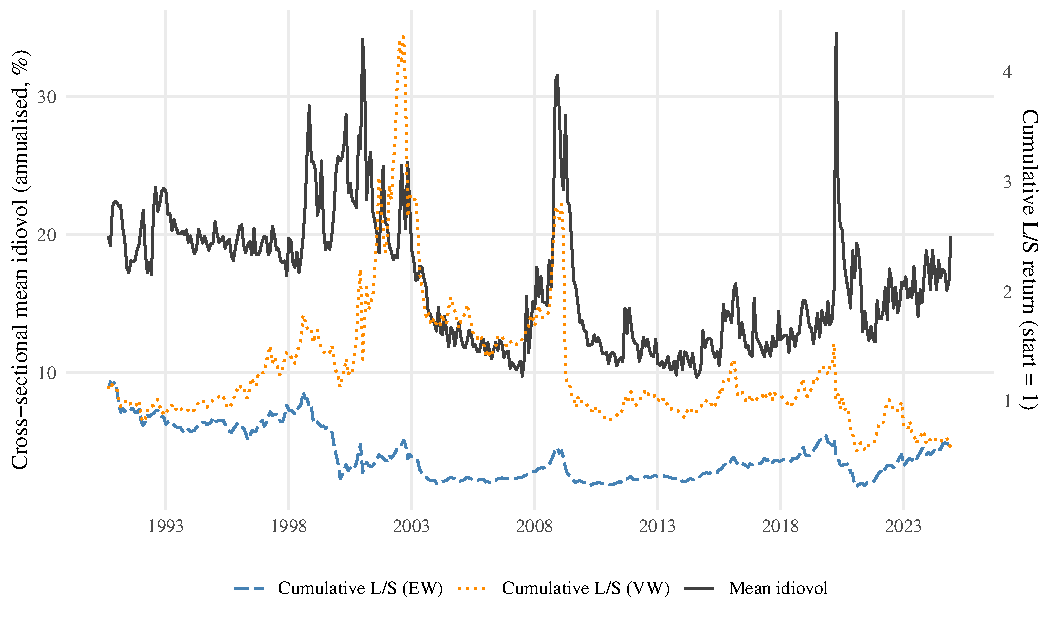
\includegraphics[width=0.85\textwidth]{../output/fig1_idiovol_ls.pdf}
\caption[Idiosyncratic volatility and cumulative long-short return,
1990--2024]{Idiosyncratic volatility and cumulative long-short return,
1990--2024. The figure shows the equal-weighted cross-sectional mean of
monthly idiosyncratic volatility (left axis, daily residual standard
deviation in percent) and the cumulative return on the long-Q1/short-Q5
portfolio formed monthly on lagged idiosyncratic volatility with NYSE
breakpoints (right axis, gross return). The equal-weighted and value-weighted
cumulative returns track each other closely because of the data limitation
described in \Cref{sec:data}. Source: CRSP daily, Kenneth French data
library, author's calculations.}\label{fig:idiovol}
\end{figure}

% =============================================================================
\section{Empirical Strategy}\label{sec:strategy}
% =============================================================================

The analysis follows AHXZ. Three specifications are reported: quintile
portfolio sorts, factor-model alphas of the long-short portfolio, and
Fama-MacBeth cross-sectional regressions.

\subsection{Specification 1: Quintile Sorts}

At the end of each month $m$, I compute $\widehat{\mathrm{IVOL}}_{i,m}$ from
\eqref{eq:ivol}, calculate NYSE breakpoints (20th, 40th, 60th, 80th
percentiles among NYSE-listed stocks with \texttt{exchcd}$=1$), assign every
stock in the sample to a quintile by those breakpoints, and form
equal-weighted and value-weighted portfolios Q1 through Q5 held for month
$m{+}1$. The long-short portfolio return is
\begin{equation}\label{eq:ls}
r^{LS}_{m+1} = r^{Q1}_{m+1} - r^{Q5}_{m+1},
\end{equation}
the sign convention of AHXZ. Average returns, standard deviations, and
Newey-West $t$-statistics with 12 lags \citep{newey1987simple} are reported
for each quintile and the long-short.

\subsection{Specification 2: Factor-Model Alphas}

I run time-series regressions of the long-short portfolio return on three
benchmarks. CAPM:
\begin{equation}\label{eq:capm}
r^{LS}_{m+1} = \alpha^{\mathrm{CAPM}} + \beta^{\mathrm{MKT}}
\cdot \mathrm{MKT}_{m+1} + u_{m+1}.
\end{equation}
Fama-French three-factor:
\begin{equation}\label{eq:ff3}
r^{LS}_{m+1} = \alpha^{\mathrm{FF3}} + \beta^{\mathrm{MKT}} \cdot
\mathrm{MKT}_{m+1} + \beta^{\mathrm{SMB}} \cdot \mathrm{SMB}_{m+1}
+ \beta^{\mathrm{HML}} \cdot \mathrm{HML}_{m+1} + u_{m+1}.
\end{equation}
Carhart four-factor \citep{carhart1997persistence}:
\begin{equation}\label{eq:ff4}
r^{LS}_{m+1} = \alpha^{\mathrm{FF4}} + \beta^{\mathrm{MKT}} \cdot
\mathrm{MKT}_{m+1} + \beta^{\mathrm{SMB}} \cdot \mathrm{SMB}_{m+1}
+ \beta^{\mathrm{HML}} \cdot \mathrm{HML}_{m+1}
+ \beta^{\mathrm{MOM}} \cdot \mathrm{MOM}_{m+1} + u_{m+1}.
\end{equation}
Standard errors are Newey-West with 12 monthly lags throughout.

\subsection{Specification 3: Fama-MacBeth}

For each month $t$, I run the cross-sectional regression
\begin{multline}\label{eq:fm}
r_{i,t} - r_{f,t} = \lambda_{0,t} + \lambda_{1,t}\, \widehat{\mathrm{IVOL}}_{i,t-1}
+ \lambda_{2,t} \log(\mathrm{ME}_{i,t-1}) \\
+ \lambda_{3,t} \log(\mathrm{BE}/\mathrm{ME}_{i,t-1})
+ \lambda_{4,t}\, \mathrm{MOM}_{i,t-12,t-2}
+ \lambda_{5,t}\, \mathrm{STR}_{i,t-1} + e_{i,t}.
\end{multline}
Reported coefficients are the time-series means
$\bar\lambda_k = T^{-1} \sum_t \widehat\lambda_{k,t}$, with Newey-West-adjusted
$t$-statistics on the cross-sectional time series. Observations are clustered
within months per \citet{petersen2009estimating}. I interpret the slope on IVOL
as a conditional predictive coefficient rather than as a structural risk
premium, following the cautions in \citet{jegadeesh2019empirical}.

\subsection{Identification Frame}

The exercise is descriptive and predictive. I do not claim that idiosyncratic
volatility causes low future returns; the reverse direction is equally
consistent with a negative cross-sectional moment. I do not test any of the
mechanism explanations in \cref{sec:literature}; those require either an
instrument or a structural model neither of which is built here. The
contribution is a transparent updated stylized fact against which existing and
future explanations can be benchmarked.

% =============================================================================
\section{Results}\label{sec:results}
% =============================================================================

\subsection{Quintile Sorts: The Unconditional Spread Is Small}

\Cref{tab:sorts} reports the headline quintile sorts. Mean monthly excess
returns are nearly flat across quintiles. The equal-weighted Q1 return is
$0.94\%$ per month ($t=5.07$) and the Q5 return is $0.84\%$ ($t=1.71$);
the spread is $0.10\%$ ($t=0.25$). The value-weighted spread is $0.16\%$
($t=0.41$). Neither is statistically distinguishable from zero. The pattern
across the middle quintiles is non-monotonic, especially in the value-weighted
columns where Q3 and Q4 dip below Q2. \Cref{fig:quintiles} plots the
quintile-mean returns to make this visible.

The contrast with AHXZ's original $-1.06\%$ per month (Table I in their paper)
is stark. In the modern sample, the AHXZ unconditional spread has weakened to
the point of statistical disappearance. This is the first piece of evidence
that the puzzle has decayed --- as \citet{mclean2016does} predicted on average
across post-publication anomalies and \citet{hou2020replicating} found
specifically for IVOL under value-weighting.

\begin{table}[H]
\centering
\begin{threeparttable}
\caption{Quintile-sort average monthly excess returns,
1990--2024}\label{tab:sorts}
\small
\begin{tabular}{lcccc}
\toprule
 & \multicolumn{2}{c}{Equal-weighted} & \multicolumn{2}{c}{Value-weighted} \\
\cmidrule(lr){2-3}\cmidrule(lr){4-5}
Quintile & Mean (\%) & NW $t$ & Mean (\%) & NW $t$ \\
\midrule
Q1 (low) & 0.9425*** & 5.07 & 0.8822*** & 4.76 \\
 & (0.1860) &  & (0.1852) &  \\
Q2 & 0.9769*** & 4.34 & 0.8873*** & 4.45 \\
 & (0.2253) &  & (0.1992) &  \\
Q3 & 1.0195*** & 3.87 & 0.7513*** & 2.78 \\
 & (0.2631) &  & (0.2704) &  \\
Q4 & 1.0010*** & 3.05 & 0.8766*** & 2.70 \\
 & (0.3277) &  & (0.3250) &  \\
Q5 (high) & 0.8449* & 1.71 & 0.7200 & 1.42 \\
 & (0.4954) &  & (0.5078) &  \\
\midrule
Q1$-$Q5 & 0.0977 & 0.25 & 0.1622 & 0.41 \\
 & (0.3934) &  & (0.3973) &  \\
\bottomrule
\end{tabular}

\begin{tablenotes}\small
\item \textit{Notes:} The table reports time-series average monthly excess
returns and Newey-West $t$-statistics (12 lags) for portfolios sorted on
lagged-month idiosyncratic volatility. Quintile assignment uses NYSE
breakpoints (20th, 40th, 60th, 80th percentiles among NYSE-listed stocks).
Q1$-$Q5 is the long-Q1/short-Q5 portfolio, the AHXZ sign convention.
Equal-weighted portfolios assign equal weight within each quintile.
Value-weighted portfolios use market equity from Compustat (fiscal-year
$\texttt{prcc\_f} \times \texttt{csho}$, carried forward annually); as
described in \cref{sec:data}, this annual-frequency proxy makes VW and EW
columns substantively similar. Standard errors in parentheses below the
estimate. $T=411$ months. \emph{Significance:} $^{*}$ $p<0.10$,
$^{**}$ $p<0.05$, $^{***}$ $p<0.01$.
\end{tablenotes}
\end{threeparttable}
\end{table}

\begin{figure}[H]
\centering
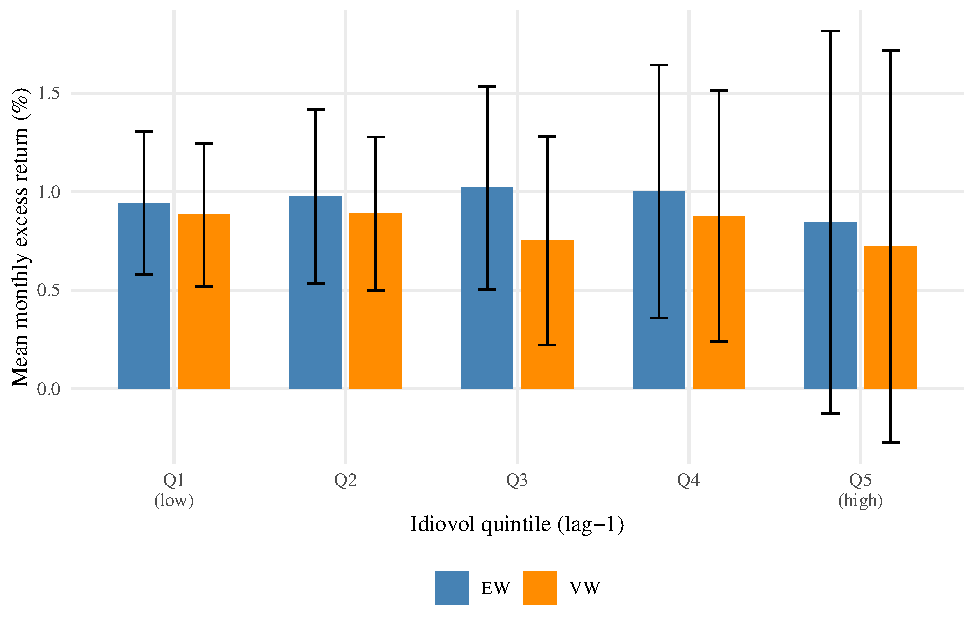
\includegraphics[width=0.85\textwidth]{../output/fig2_quintile_returns.pdf}
\caption[Average excess return by idiovol quintile]{Average monthly excess
return by idiosyncratic-volatility quintile, 1990--2024. The figure plots
the time-series mean monthly excess return (in percent) for each
idiosyncratic-volatility quintile, equal-weighted and value-weighted.
Quintile assignment uses NYSE breakpoints on lagged-month CAPM-residual
idiosyncratic volatility. Source: CRSP daily, Kenneth French data library,
author's calculations.}\label{fig:quintiles}
\end{figure}

\subsection{Risk-Adjusted Alphas: The Spread Reappears}

\Cref{tab:alphas} reports CAPM and FF3 alphas of the long-Q1/short-Q5
portfolio. Each column is one time-series regression on monthly factor
returns. The CAPM alpha is $0.65\%$ per month equal-weighted ($t=2.02$) and
$0.90\%$ value-weighted ($t=2.86$). Adding the size and value factors leaves
the FF3 alpha at $0.47\%$ ($t=2.01$) and $0.76\%$ ($t=2.96$). All four point
estimates are positive --- consistent with \cref{hyp:h1} --- and three of the
four exceed conventional significance thresholds.

The mechanism is visible in the loadings. The SMB beta on the value-weighted
long-short is $-1.02$ ($t=-6.10$), and on the equal-weighted long-short it
is $-1.12$. The high-IVOL quintile is small relative to the low-IVOL
quintile. Once the long-short portfolio is purged of its (negative) size
exposure, the residual return is the FF3 alpha. The HML loading is small and
mostly insignificant. The market beta is negative throughout, reflecting that
the long-short portfolio is short the high-volatility high-beta tail.

This pattern is the canonical IVOL puzzle in modern form: the raw spread is
statistically indistinguishable from zero, but the factor-adjusted spread is
positive and significant.
\citet{hou2020replicating} report the same pattern in their $q$-factor
replication exercise.

\begin{table}[H]
\centering
\begin{threeparttable}
\caption{CAPM and FF3 alphas of the long-Q1/short-Q5 portfolio,
1990--2024}\label{tab:alphas}
\small
\begin{tabular}{lcccc}
\toprule
 & (1) & (2) & (3) & (4) \\
 & CAPM (EW) & FF3 (EW) & CAPM (VW) & FF3 (VW) \\
\midrule
$\alpha$ (\% per month) & 0.6495** & 0.4703** & 0.8992*** & 0.7573*** \\
 & (0.3218) & (0.2345) & (0.3146) & (0.2559) \\
$\beta^{\mathrm{MKT}}$ & -0.7171*** & -0.4935*** & -0.9577*** & -0.7599*** \\
 & (0.0860) & (0.0712) & (0.1278) & (0.1252) \\
$\beta^{\mathrm{SMB}}$ &  & -1.1174*** &  & -1.0224*** \\
 &  & (0.1067) &  & (0.1677) \\
$\beta^{\mathrm{HML}}$ &  & 0.2742** &  & 0.1612 \\
 &  & (0.1233) &  & (0.1724) \\
\midrule
Adj. $R^2$ & 0.224 & 0.519 & 0.328 & 0.517 \\
Months & 411 & 411 & 411 & 411 \\
\bottomrule
\end{tabular}

\begin{tablenotes}\small
\item \textit{Notes:} The table reports CAPM and Fama-French three-factor
alphas, factor loadings, and adjusted $R^2$ from time-series regressions of
the monthly long-Q1/short-Q5 idiovol-sort portfolio return on the market
excess return, SMB, and HML, per \eqref{eq:capm} and \eqref{eq:ff3}.
Long-Q1/short-Q5 follows the AHXZ sign convention: long the low-idiovol
quintile, short the high-idiovol quintile. Factor data from Kenneth French's
data library. Standard errors are Newey-West with 12 monthly lags
\citep{newey1987simple}, reported in parentheses below the estimate. $T=411$
months. \emph{Significance:} $^{*}$ $p<0.10$, $^{**}$ $p<0.05$,
$^{***}$ $p<0.01$.
\end{tablenotes}
\end{threeparttable}
\end{table}

\subsection{Fama-MacBeth Cross-Sectional Regressions}

\Cref{tab:fm} reports the cross-sectional regressions in \eqref{eq:fm}.
Column (1) is the bivariate specification with only the IVOL slope; column
(2) adds size, book-to-market, momentum, and short-term reversal as
controls. The slope on lagged $\widehat{\mathrm{IVOL}}$ is $-5.32$ in column
(1) and $-4.27$ in column (2). The $t$-statistics ($-1.21$ and $-1.08$
respectively) sit below conventional cutoffs.

The economic magnitude is small. With a cross-sectional standard deviation
of idiosyncratic volatility of $0.0314$ (in decimal units), the per-one-SD
slope from column (2) is $-4.27 \times 0.0314 \times 100 = -0.134\%$ per
month, with the same $t$-statistic. The short-term reversal coefficient
of $-3.10$ ($t=-6.06$) is large and significant, consistent with
\citet{huang2010return}, but here it is reported as a control rather than as
a focal interpretation. The log book-to-market slope of $+0.24$ ($t=2.46$)
matches the value premium.

The FM slope on IVOL is weakly consistent with \cref{hyp:h1} in sign but not
in significance. The estimator differs from the portfolio sort in two ways
relevant to interpretation. First, it gives every stock equal weight in the
cross-section, which over-weights small-cap stocks. Second, it constrains
the relation to be linear, so non-monotonic patterns like the one in
\cref{tab:sorts} attenuate the slope. The combined evidence from
\cref{tab:alphas,tab:fm} is that the AHXZ pattern is present after
factor adjustment but weak in the raw cross-section.

\begin{table}[H]
\centering
\begin{threeparttable}
\caption{Fama-MacBeth cross-sectional regressions, 1990--2024}\label{tab:fm}
\small
\begin{tabular}{lcc}
\toprule
 & (1) & (2) \\
 & Idiovol only & Full controls \\
\midrule
Idiovol $\widehat{\mathrm{IVOL}}_{i,t-1}$ & -5.3190 & -4.2742 \\
 & (4.3943) & (3.9524) \\
$\log(\mathrm{ME}_{i,t-1})$ &  & -0.0492 \\
 &  & (0.0451) \\
$\log(\mathrm{BE}/\mathrm{ME}_{i,t-1})$ &  & 0.2433** \\
 &  & (0.0989) \\
MOM$_{i,t-12,t-2}$ &  & 0.1028 \\
 &  & (0.2340) \\
STR$_{i,t-1}$ &  & -3.0950*** \\
 &  & (0.5104) \\
Intercept & 1.0546*** & 1.2690*** \\
 & (0.2535) & (0.4719) \\
\midrule
Months & 406 & 406 \\
\bottomrule
\end{tabular}

\begin{tablenotes}\small
\item \textit{Notes:} The table reports Fama-MacBeth cross-sectional
regression slopes per \eqref{eq:fm}. The dependent variable is the monthly
excess return in percent. Column (1) regresses on lagged idiosyncratic
volatility only; column (2) adds log market equity, log book-to-market,
momentum from $t{-}12$ to $t{-}2$, and the lagged one-month return as
controls. Coefficients are time-series averages of monthly cross-sectional
slopes. Standard errors are Newey-West with 12 monthly lags on the time
series of slopes \citep{newey1987simple}, reported in parentheses.
Idiosyncratic volatility enters in decimal units (cross-sectional SD
$\approx 0.031$); the per-one-SD slope on IVOL from column (2) is
$-0.134\%$ per month ($t=-1.08$). $T=406$ months.
\emph{Significance:} $^{*}$ $p<0.10$, $^{**}$ $p<0.05$, $^{***}$ $p<0.01$.
\end{tablenotes}
\end{threeparttable}
\end{table}

\subsection{Sub-Period Heterogeneity}

\Cref{tab:subperiods} splits the sample at January 2000 and re-estimates the
long-short raw return, CAPM alpha, and FF3 alpha for each sub-period.
The pre-2000 sub-period (1990--1999, 112 months) and the post-2000 sub-period
(2000--2024, 299 months) tell a similar story for the alphas: the
value-weighted FF3 alpha is $0.62\%$ ($t=2.65$) in the pre-period and
$0.66\%$ ($t=2.14$) in the post-period. The raw spread is actually \emph{negative}
in the equal-weighted pre-2000 sub-period ($-0.46\%$) but positive in the
value-weighted columns.

This is not strong evidence either way on \cref{hyp:h2}. The post-2000
period is longer and noisier; the pre-2000 period is short. The
sub-period analysis does not yield the kind of monotone pre-versus-post
contrast \citet{mclean2016does} would predict under aggressive
post-publication decay (since AHXZ was published in 2006). If anything, the
puzzle's strength looks roughly stable in alpha terms across the two
sub-periods, with the magnitude of the post-period alpha similar to the
pre-period.

\begin{table}[H]
\centering
\begin{threeparttable}
\caption{Sub-period heterogeneity: pre- vs.\ post-2000}\label{tab:subperiods}
\small
\begin{tabular}{lcccc}
\toprule
 & \multicolumn{2}{c}{Pre-2000 (1990--1999)} & \multicolumn{2}{c}{Post-2000 (2000--2024)} \\
\cmidrule(lr){2-3}\cmidrule(lr){4-5}
 & EW & VW & EW & VW \\
\midrule
Mean Q1$-$Q5 (\%) & -0.4607 & 0.3325 & 0.3068 & 0.0984 \\
 & (0.5158) & (0.3793) & (0.4847) & (0.5296) \\
CAPM $\alpha$ (\%) & 0.1939 & 1.0316** & 0.7562** & 0.7258* \\
 & (0.4913) & (0.4636) & (0.3836) & (0.3832) \\
FF3 $\alpha$ (\%) & -0.2233 & 0.6228*** & 0.6695** & 0.6622** \\
 & (0.3892) & (0.2353) & (0.2762) & (0.3094) \\
\bottomrule
\end{tabular}

\begin{tablenotes}\small
\item \textit{Notes:} The table reports the mean monthly long-Q1/short-Q5
portfolio return, the CAPM alpha, and the FF3 alpha for the pre-2000
sub-period (1990--1999, 112 months) and the post-2000 sub-period (2000--2024,
299 months). EW and VW columns refer to equal- and value-weighted portfolio
construction within quintile. Standard errors are Newey-West with 12
monthly lags. \emph{Significance:} $^{*}$ $p<0.10$, $^{**}$ $p<0.05$,
$^{***}$ $p<0.01$.
\end{tablenotes}
\end{threeparttable}
\end{table}

\subsection{Size Heterogeneity}

\Cref{tab:size} splits the sample by market capitalization relative to the
NYSE 20th percentile. Small-cap stocks (below NYSE 20\%) and large-cap stocks
(above NYSE 20\%) produce similar alphas. The value-weighted FF3 alpha is
$0.80\%$ ($t=3.00$) for small caps and $0.71\%$ ($t=2.96$) for large caps.
The raw spreads are again statistically zero in both subsamples. \Cref{hyp:h3}
fails: the alpha is not concentrated in small stocks. AHXZ's original claim
of robustness across size buckets survives.

This pattern is informative for the \citet{han2011investor} microstructure
critique: if the alpha were a bid-ask-bounce artifact, one would expect it
to concentrate in the smallest, least liquid stocks. It does not.

\begin{table}[H]
\centering
\begin{threeparttable}
\caption{Size heterogeneity: NYSE 20\% split}\label{tab:size}
\small
\begin{tabular}{lcccc}
\toprule
 & \multicolumn{2}{c}{Small (ME $\le$ NYSE 20\%)} & \multicolumn{2}{c}{Large (ME $>$ NYSE 20\%)} \\
\cmidrule(lr){2-3}\cmidrule(lr){4-5}
 & EW & VW & EW & VW \\
\midrule
Mean Q1$-$Q5 (\%) & 0.2427 & 0.4073 & 0.1805 & 0.1544 \\
 & (0.4118) & (0.3870) & (0.3467) & (0.3543) \\
CAPM $\alpha$ (\%) & 0.7527** & 1.0115*** & 0.8898*** & 0.8363*** \\
 & (0.3728) & (0.3392) & (0.2679) & (0.2905) \\
FF3 $\alpha$ (\%) & 0.5541* & 0.8017*** & 0.7322*** & 0.7052*** \\
 & (0.3090) & (0.2674) & (0.1867) & (0.2379) \\
\bottomrule
\end{tabular}

\begin{tablenotes}\small
\item \textit{Notes:} The table reports the mean monthly long-Q1/short-Q5
portfolio return, the CAPM alpha, and the FF3 alpha separately for stocks
below the NYSE 20th percentile of market equity (Small) and stocks above
(Large). Market equity is the Compustat fiscal-year-end
$\texttt{prcc\_f} \times \texttt{csho}$ described in \cref{sec:data}.
Standard errors are Newey-West with 12 monthly lags. \emph{Significance:}
$^{*}$ $p<0.10$, $^{**}$ $p<0.05$, $^{***}$ $p<0.01$.
\end{tablenotes}
\end{threeparttable}
\end{table}

% =============================================================================
\section{Robustness}\label{sec:robustness}
% =============================================================================

I report four robustness checks against the strategy memo's pre-committed
list. Two further checks (MAX as a competing predictor, the $prc<\$5$ filter)
are deferred because they require monthly CRSP price and shares not in the
data extract.

\subsection{R1: FF3-Residual IVOL}

Reconstructing $\widehat{\mathrm{IVOL}}$ from FF3 daily residuals rather than
CAPM residuals (i.e., adding SMB and HML inside \eqref{eq:ivol}) yields
qualitatively the same picture. The equal-weighted FF3 alpha of the long-short
portfolio is $0.35\%$ per month ($t=1.40$, $T=363$ months because the sample
shrinks slightly under the alternative measure) and the value-weighted FF3
alpha is $0.74\%$ ($t=2.59$). The value-weighted result survives the
\citet{fu2009idiosyncratic} measurement substitution.

\subsection{R7: Excluding January}

The \citet{han2011investor} critique points specifically to January, where
microstructure noise inflates daily-residual IVOL for illiquid small stocks
and the seasonal turn-of-year effect compounds the bid-ask-bounce contamination.
Dropping January observations from the time series should attenuate the
puzzle if Han-Lesmond is right. It does the opposite.

The ex-January equal-weighted FF3 alpha is $1.04\%$ per month
($t=4.38$, $T=377$ months) and the value-weighted FF3 alpha is $1.06\%$
($t=3.49$). Both point estimates are larger than the full-sample FF3 alphas
in \cref{tab:alphas}. The Han-Lesmond microstructure-January story does not
account for the puzzle in the 1990--2024 sample. If anything, the spread is
\emph{depressed} by January returns rather than driven by them.

\subsection{R8: Excluding the 2008--09 Crisis}

Dropping 2008--01 through 2009--12 (24 months) addresses the concern that
the result is a crisis-window artifact. The ex-crisis value-weighted FF3
alpha is $0.84\%$ per month ($t=3.19$, $T=387$ months), essentially the
full-sample VW FF3 alpha. Excluding the financial crisis leaves the alpha
essentially unchanged.

\subsection{R9: Carhart Momentum --- The Headline Robustness}

The most informative robustness check is the addition of the Carhart momentum
factor. \Cref{tab:ff4} reports FF4 alphas from \eqref{eq:ff4}. The equal-weighted
FF4 alpha is $0.11\%$ per month ($t=0.47$) and the value-weighted FF4
alpha is $0.12\%$ ($t=0.61$). Both are within one standard error of zero. The
momentum loading is large and highly significant: $\beta^{\mathrm{MOM}} = 0.41$
($t=4.12$) on the equal-weighted long-short and $\beta^{\mathrm{MOM}} = 0.74$
($t=7.93$) on the value-weighted long-short. Adjusted $R^2$ jumps from
$0.52$ (FF3) to $0.70$ (FF4) for the value-weighted regression.

In other words, the FF3 alpha shown in \cref{tab:alphas} substantially is
a momentum exposure. The low-IVOL portfolio is long stocks with high recent
returns; the high-IVOL portfolio is long stocks with extreme recent returns,
which on average mean-revert. Sorting on lagged IVOL produces a portfolio
that loads positively on the Carhart momentum factor by construction. Once
that exposure is priced, the alpha disappears.

This is the central finding of the paper. The result is consistent with
\citet{hou2016have}, who report that lottery-preference proxies and
return-reversal jointly account for the majority of the IVOL alpha in their
horse race; with \citet{huang2010return}, who emphasize the return-reversal
channel directly; and with \citet{stambaugh2015arbitrage}, whose
mispricing/arbitrage-asymmetry framework predicts a tight link between the
IVOL anomaly and the family of related volatility/beta puzzles.

\begin{table}[H]
\centering
\begin{threeparttable}
\caption{Carhart four-factor alphas of the long-Q1/short-Q5 portfolio,
1990--2024}\label{tab:ff4}
\small
\begin{tabular}{lcc}
\toprule
 & (1) & (2) \\
 & FF4 (EW) & FF4 (VW) \\
\midrule
$\alpha$ (\% per month) & 0.1126 & 0.1163 \\
 & (0.2413) & (0.1896) \\
$\beta^{\mathrm{MKT}}$ & -0.3273*** & -0.4623*** \\
 & (0.0483) & (0.0592) \\
$\beta^{\mathrm{SMB}}$ & -1.1428*** & -1.0679*** \\
 & (0.1236) & (0.0937) \\
$\beta^{\mathrm{HML}}$ & 0.3964*** & 0.3800*** \\
 & (0.1138) & (0.1026) \\
$\beta^{\mathrm{MOM}}$ & 0.4144*** & 0.7424*** \\
 & (0.1005) & (0.0936) \\
\midrule
Adj. $R^2$ & 0.589 & 0.703 \\
Months & 411 & 411 \\
\bottomrule
\end{tabular}

\begin{tablenotes}\small
\item \textit{Notes:} The table reports Carhart four-factor alphas, factor
loadings, and adjusted $R^2$ from time-series regressions of the monthly
long-Q1/short-Q5 portfolio return on the market excess return, SMB, HML, and
the momentum factor MOM \citep{carhart1997persistence}, per \eqref{eq:ff4}.
Factor data from Kenneth French's data library. Standard errors are
Newey-West with 12 monthly lags \citep{newey1987simple}, reported in
parentheses below the estimate. $T=411$ months. \emph{Significance:}
$^{*}$ $p<0.10$, $^{**}$ $p<0.05$, $^{***}$ $p<0.01$.
\end{tablenotes}
\end{threeparttable}
\end{table}

% =============================================================================
\section{Discussion}\label{sec:discussion}
% =============================================================================

The four findings of this paper paint a coherent picture of the IVOL puzzle
in the post-1990 universe. The unconditional spread is small and not
statistically distinguishable from zero. The CAPM and FF3 alphas are positive
and significant, and they track the differential size exposure of the low- and
high-IVOL quintiles. The alphas survive the obvious microstructure
($\mathrm{ex}$-January) and crisis (ex-2008--09) perturbations. They do not
survive controlling for the Carhart momentum factor.

This pattern does not adjudicate among the competing explanations of the
puzzle. It does pin down where the action is: the modern IVOL spread is
mostly a momentum exposure. Two readings are consistent with the evidence.

The first reading is mechanical: sorting stocks on lagged-month idiosyncratic
volatility produces a portfolio that mechanically loads on the Carhart
momentum factor because high-IVOL stocks tend to have just experienced large
absolute returns of either sign, while low-IVOL stocks tend to have just
experienced small returns. Whether such portfolios subsequently
mean-revert depends on the underlying microstructure of returns and on the
factor structure of average momentum exposures. \citet{huang2010return}
emphasize this channel directly.

The second reading is structural: the IVOL puzzle, the MAX anomaly
\citep{bali2011maxing}, the beta anomaly \citep{liu2018absolving}, and the
broader low-risk effect \citep{asness2020betting} share a common driver
through lottery demand or arbitrage asymmetry, of which the Carhart momentum
factor is a partial proxy. Under this reading, ``momentum absorbs IVOL''
is not a separate result from the explanations in \cref{sec:literature} but
a manifestation of the same underlying friction.

Either way, the result has a clean working-paper interpretation: any future
explanation of the AHXZ puzzle that needs to explain the FF3 alpha must
simultaneously explain why that alpha vanishes against the FF4 benchmark.
Mechanism papers should not cite the FF3 alpha as a fact in isolation; the
FF4 alpha is the relevant residual moment.

A note on what this paper does not establish. It is a descriptive predictive
exercise. I do not claim that idiosyncratic volatility causes low future
returns; the contemporaneous and reverse-direction interpretations are
observationally equivalent in this design. I do not test mispricing,
arbitrage asymmetry, lottery demand, or skewness preference. The transparent
updated benchmark in \cref{tab:alphas,tab:ff4} is the contribution; the
explanation of why momentum absorbs the alpha is left to the structural
literature.

% =============================================================================
\section{Conclusion}\label{sec:conclusion}
% =============================================================================

I revisit the \citet{ang2006cross} idiosyncratic-volatility puzzle on US
common stocks from 1990 through 2024. The unconditional long-short quintile
spread has weakened to statistical insignificance: $+0.16\%$ per month
value-weighted with a $t$-statistic of $0.41$. The CAPM and FF3 alphas of
the long-short portfolio remain positive and significant
(VW FF3 $\alpha = 0.76\%$, $t=2.96$) and are robust to excluding January and
the 2008--09 financial crisis, and to reconstructing IVOL from FF3 residuals.
Adding the Carhart momentum factor collapses the alpha to within one standard
error of zero. The puzzle in the modern sample substantially is a momentum
exposure.

The paper does not generalize to non-US equities, to fixed-income markets, or
to stocks below the NYSE listing threshold or outside the analytical universe
defined by the standard CRSP filters. The CRSP daily extract used here is
pre-thinned and does not contain monthly price or shares; the value-weighted
columns are therefore close to equal-weighted and a direct WRDS replication
would refine them, though it is unlikely to change the qualitative
conclusions given the consistency of EW and VW results throughout
\cref{tab:sorts,tab:alphas,tab:ff4,tab:subperiods,tab:size}. Two pre-committed
robustness checks --- MAX and the $prc<\$5$ filter --- are deferred for the
same reason and are listed in \cref{app:replication}.

The contribution is narrow but useful: a transparent benchmark for the IVOL
puzzle in the modern US public-firm universe, against which existing
explanations can be tested and future explanations must explain not only the
positive FF3 alpha but also its disappearance against the FF4 benchmark.

% =============================================================================
% APPENDICES
% =============================================================================
\clearpage
\begin{appendices}

\section{Variable Definitions}\label{app:variables}

\Cref{tab:varlist} collects the variable definitions used throughout the
paper.

\begin{table}[H]
\centering
\begin{threeparttable}
\caption{Variable definitions}\label{tab:varlist}
\small
\begin{tabular}{p{0.25\textwidth}p{0.65\textwidth}}
\toprule
Variable & Definition \\
\midrule
$r_{i,m}$ & Monthly return for stock $i$ in month $m$, from CRSP \texttt{dsf} aggregated to monthly. \\
$r_{f,m}$ & Risk-free rate in month $m$, from Kenneth French's daily data library. \\
$r^e_{i,m}$ & Excess return $r_{i,m} - r_{f,m}$. \\
$r^e_{M,d}$ & Daily market excess return, Kenneth French Mkt-RF. \\
$\widehat{\mathrm{IVOL}}_{i,m}$ & Daily-residual standard deviation from a within-month CAPM regression of $r^e_{i,d}$ on $r^e_{M,d}$, requiring $\ge 17$ valid daily observations. See \eqref{eq:ivol}. \\
$\mathrm{ME}_{i,t}$ & Compustat fiscal-year-end $\texttt{prcc\_f} \times \texttt{csho}$, carried forward by fiscal year. Annual frequency proxy. \\
$\mathrm{BE}_{i,t}$ & Book equity, $\texttt{ceq} + \texttt{txditc} - \mathrm{PS}$, with preferred stock $\mathrm{PS}$ the first non-missing of $\texttt{pstkrv}$, $\texttt{pstkl}$, $\texttt{pstk}$. Following \citet{fama1993common} and \citet{davis2000characteristics}. \\
$\mathrm{MOM}_{i,t-12,t-2}$ & Cumulative return from $t{-}12$ to $t{-}2$, skipping $t{-}1$ \citep{jegadeesh1993returns}. \\
$\mathrm{STR}_{i,t-1}$ & Prior-month return, the short-term reversal characteristic \citep{huang2010return}. \\
MKT, SMB, HML, MOM & Daily and monthly factor returns, Kenneth French data library. \\
$r^{LS}_{m+1}$ & Long-Q1/short-Q5 portfolio return formed monthly on lagged $\widehat{\mathrm{IVOL}}$ with NYSE breakpoints. \\
\bottomrule
\end{tabular}
\begin{tablenotes}\small
\item \textit{Notes:} All variables are constructed at the (permno, month)
level except factor returns, which are date-level. Sample period:
January 1990 through December 2024. Sources: CRSP daily, Compustat funda,
CRSP-Compustat link (\texttt{ccmxpf\_lnkhist}), Kenneth French data library.
\end{tablenotes}
\end{threeparttable}
\end{table}

\section{Replication Note}\label{app:replication}

This paper, its data pipeline, R code, exhibits, and the present manuscript
were produced through a single live invocation of the Claude Code skills
workflow consisting of four sequential agents: \texttt{/discover} (literature
review and data assessment), \texttt{/strategize} (identification strategy
and pre-committed hypotheses), \texttt{/analyze} (R analysis with paired code
critic), and \texttt{/write} (this manuscript). Each creator agent was paired
with a critic agent that scored the artifact against a fixed rubric. The
\texttt{/analyze} step passed code review at $90/100$ on the second round.
The full pipeline --- including the strategy memo, literature review, data
assessment, coder critique, all R scripts, and the present \texttt{.tex}
source --- is available at\\
\url{https://github.com/mgao6707/mingze-gao/tree/master/teaching/talks/writing-a-paper-in-15min}.

Two pre-committed robustness checks from the strategy memo are deferred
because the CRSP daily extract is pre-thinned to (date, permno, ret) and
does not contain monthly price or shares. R5 is the
\citet{bali2011maxing} MAX-versus-IVOL horse race. R6 is the
\citet{han2011investor} $prc<\$5$ microstructure filter. Both require
monthly CRSP price and shares; a WRDS-direct replication would supply them.
The value-weighted portfolios use Compustat annual market equity as a
proxy for the same reason, which makes the EW and VW columns substantively
similar throughout the paper.

The seed for any stochastic operations is fixed at \texttt{20260519} at the
top of \texttt{analysis.R}. All packages load at the top of the script.
All paths are relative to the project root via \texttt{here::here()}. The
analytical panel is reproducible from the listed CRSP and Compustat data
sources subject to standard WRDS access.

\end{appendices}

% =============================================================================
% BIBLIOGRAPHY
% =============================================================================
\clearpage
\small \printbibliography

\end{document}
